\section{Cathode-Anode Correlation}

\label{sec:lct}

\subsection{LCT Algorithm}
\label{subsec:lct_algo}

The Trigger Motherboard (TMB) portion of the CLCT/TMB card receives up to two
anode stubs from the ALCT board and two cathode stubs from the CLCT portion of the CLCT/
TMB card. The functions of the TMB circuitry are:

\begin{itemize}
	\item Bunch crossing alignment of the anode and cathode tags.
	\item Correlation of the Anode and Cathode LCT words and construction of two combined LCTs.
	\item Transmission of LCT data to the Muon Port Card (MPC) for triggering, and transmission of DAQ data to the DAQ Motherboard (DAQMB).
\end{itemize}

Incoming anode and cathode LCTs are not aligned in time. Anode LCTs are created
faster than cathode LCTs because of the slow development of the cathode preamp signal, and
because processing inside the ALCT card is faster than processing inside the CLCT logic. The
TMB contains input pipeline logic in order to delay anode LCTs for a programmable number of
bunch crossings up to 10.

The anode and cathode LCTs are matched according to the more precise ALCT bunch
crossing number (BXN). The Cathode LCT BXN can differ by at most $\pm$1 bunch crossing. For each
of the selected muons the TMB outputs a 2-bit bunch crossing match word as shown in
table below. These may be used by later boards in the trigger chain if additional quality information
is needed. They also allow the analysis of the bunch crossing matching in the TMB, since a large
number of bad matches could be an indication of a timing alignment problem.

The ideal case for a high-momentum muon is one anode and one cathode LCT pattern.
However, other cases may occur, which are distinguished by a 2-bit “STA” (Status type A) code:

\begin{itemize}
	\item The TMB may receive one or two anode LCTs and zero cathode LCT patterns. This
happens, for example, for very low-momentum muons. Although the non-zero data is
forwarded to the MPC, this case is flagged by STA=1, as is the similar case of one or two
cathode LCT and zero anode LCT patterns.
	\item If the TMB receives two anode LCTs and one cathode LCT, the TMB outputs two LCTs,
by copying the Cathode LCT bits into both muons. These, and the similar case of two
cathode LCTs and one anode LCT, are flagged by STA=2.
	\item If there are two anode LCTs and two cathode LCTs in one chamber, they are matched
according to their pattern numbers: the largest ALCT and CLCT pattern numbers are
paired, and the second largest ALCT and CLCT pattern numbers are paired. These, and
the ideal case of a single match, are flagged by STA=3.
\end{itemize}

TMBs maintain a local Bunch Crossing Number (BXN) using signals from the Clock
and Control Board. The internal BXN is compared to the BXN received from the ALCT module,
and the Sync Error bit is set if a mismatch is detected.

The TMB sends up to two anode LCT and two cathode LCT patterns for one CSC
chamber to the MPC every 25 ns.

\subsection{Reduction of the Matching Time Window}

The current TMB uses a rather wide time matching window (7BX) that is centered on a CLCT's BX, and is used to look for an ALCT match within it. A wide matching window is not good in high pileup, as propability of incorrect matching with background 2D stubs is higher, resulting in inefficiency.

For the SLHC, we can probably assume that the system is well timed and that we can use the narrowest reasonable matching window of 3BX wide (see "matchTrigWindowSize" parameter in Sec.~\ref{sec:TMB_conf}). 

\subsection{Modification of the Stub Timing Logic in Matching}

 In the old TMB algorithm, the stub timing logic works during the 2D stubs matching as follows:
\begin{itemize}
    \item CLCT-centric approach: CLCTs and their BX are taken as reference points, while ALCTs are waiting in a queue
    \item for a BX with CLCTs we look for a first BX in the matching window that has ALCTs
    \item after matching is dome in this BX, the ALCTs from there are taken off the queue, and cannot be matched with any later CLCT (see "tmbDropUsedClcts" and "matchEarliestClctME11Only" parameters in Sec.~\ref{sec:TMB_conf})
\end{itemize}

The main issues with this approach at high luminosity is that when there is an ALCT from a good signal muon, early CLCTs from background might steal it and form wrong match, and this correct ALCT then would not be available anymore for matching with a later correct CLCT.

Proposal to improve the situation:
\begin{itemize}
    \item ALCT-centric approach: ALCTs and their BXs are taken as reference points, while reconstructed CLCTs are waiting in a matching window-wide queue (see "clctToAlct" parameter in Sec.~\ref{sec:TMB_conf})
    \begin{itemize}
        \item ALCT's BX and the middle BX in the matching window-wide queue are expected to be synchronized 
    \end{itemize}
    \item for an ALCT's BX we look for CLCTs within the queue in the order of arrival try to find maximum 2 LCT matches as follows (see "tmbCrossBxAlgorithm" parameter in Sec.~\ref{sec:TMB_conf}):
    \begin{itemize}
        \item first look for CLCTs in the same BX 2) if we didn't get 2 LCT matches yet, look for CLCTs in BX-1
        \item if we didn't get 2 LCT matches yet, look for CLCTs in BX+1
        \item etc... depending on how wide the matching window is 
    \end{itemize}
    \item can optionally either remove CLCTs from the queue after there was an LCT match, or can keep them for reuse possibilities to be matched with later ALCTs (see "tmbDropUsedClcts" parameter in Sec.~\ref{sec:TMB_conf})
    \item NOTE: all this is supposed to be done separately in ME1/1a and in ME1/1b 
\end{itemize}

\subsection{Selection of the Two Best LCTs per ME1/1}

With the backplane limitations, we can read out only up to two trigger stubs per BX from the whole ME1/1.

Since ME1/1a and ME1/1b now can each have up to two stubs, we need an extra step of selecting the best two ME1/1 stubs out of possible 4. If ME1/1a + ME1/1b has more then two LCTs:
\begin{itemize}
    \item The simplest solution:
    \begin{itemize}
	\item drop the highest eta ones until we have just two. 
    \end{itemize}
    \item Possible improvement:
    \begin{itemize}
        \item rank stubs by special quality value which is the same as stub quality for ME1/1b and is stub quality-1 for ME1/1a stubs
        \item if special quality is the same, rank by eta 
    \end{itemize}
\end{itemize}

\newpage
\subsection{Software Emulation of CLCT and ALCT Matching}

Every BX OTMB receives up to 2 CLCTs and up to two ALCTs from CLCT and ALCT processors, Fig.~\ref{fig:clcts_alcts} shows an example which will be used throughout the subsection.

\begin{figure}[tbh]
        \begin{center}
                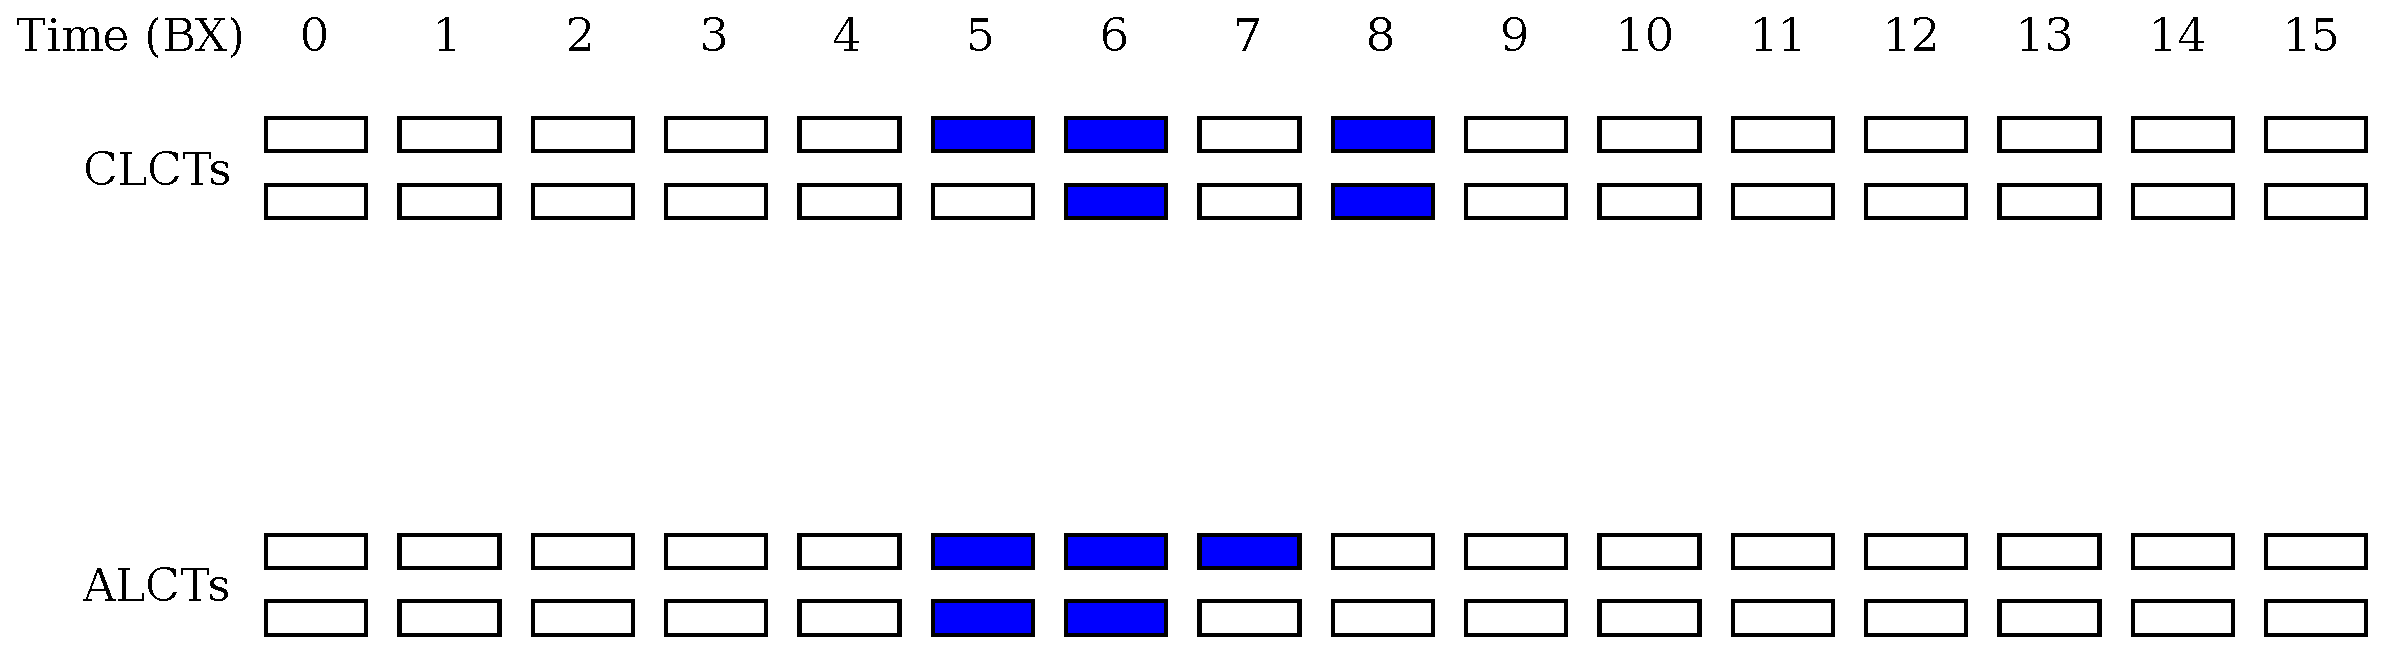
\includegraphics[width=0.7\linewidth]{figures/clcts_alcts.pdf}
                \caption{Example of CLCTs and ALCTs received by OTMB.}
                \label{fig:clcts_alcts}
        \end{center}
\end{figure}

There are two approaches to CLCT and ALCT correlation: CLCT-centric and ALCT-centric. We will introduce the former below and discuss the latter later among OTMB level improvements.

CLCT-centric CLCT and ALCT correlation (see Fig.~\ref{fig:clct_alcts}):
\begin{itemize}
    \item Loop over CLCT BXs from BX = 0 to BX = 15
    \item For CLCT BX = B with at least one valid CLCT:
    \begin{itemize}
        \item Loop over ALCT BXs from BX = B-3 to BX = B+3
        \item Find the first ALCT BX in the matching window with at least one valid ALCT and not marked as used before
        \begin{itemize}
            \item Correlate CLCTs and ALCTs in matching ALCT and CLCT BXs
            \item Mark ALCT BX as used
            \item Proceed to next CLCT BX
        \end{itemize}
    \end{itemize}
\end{itemize}

\begin{figure}[tbh]
        \begin{center}
                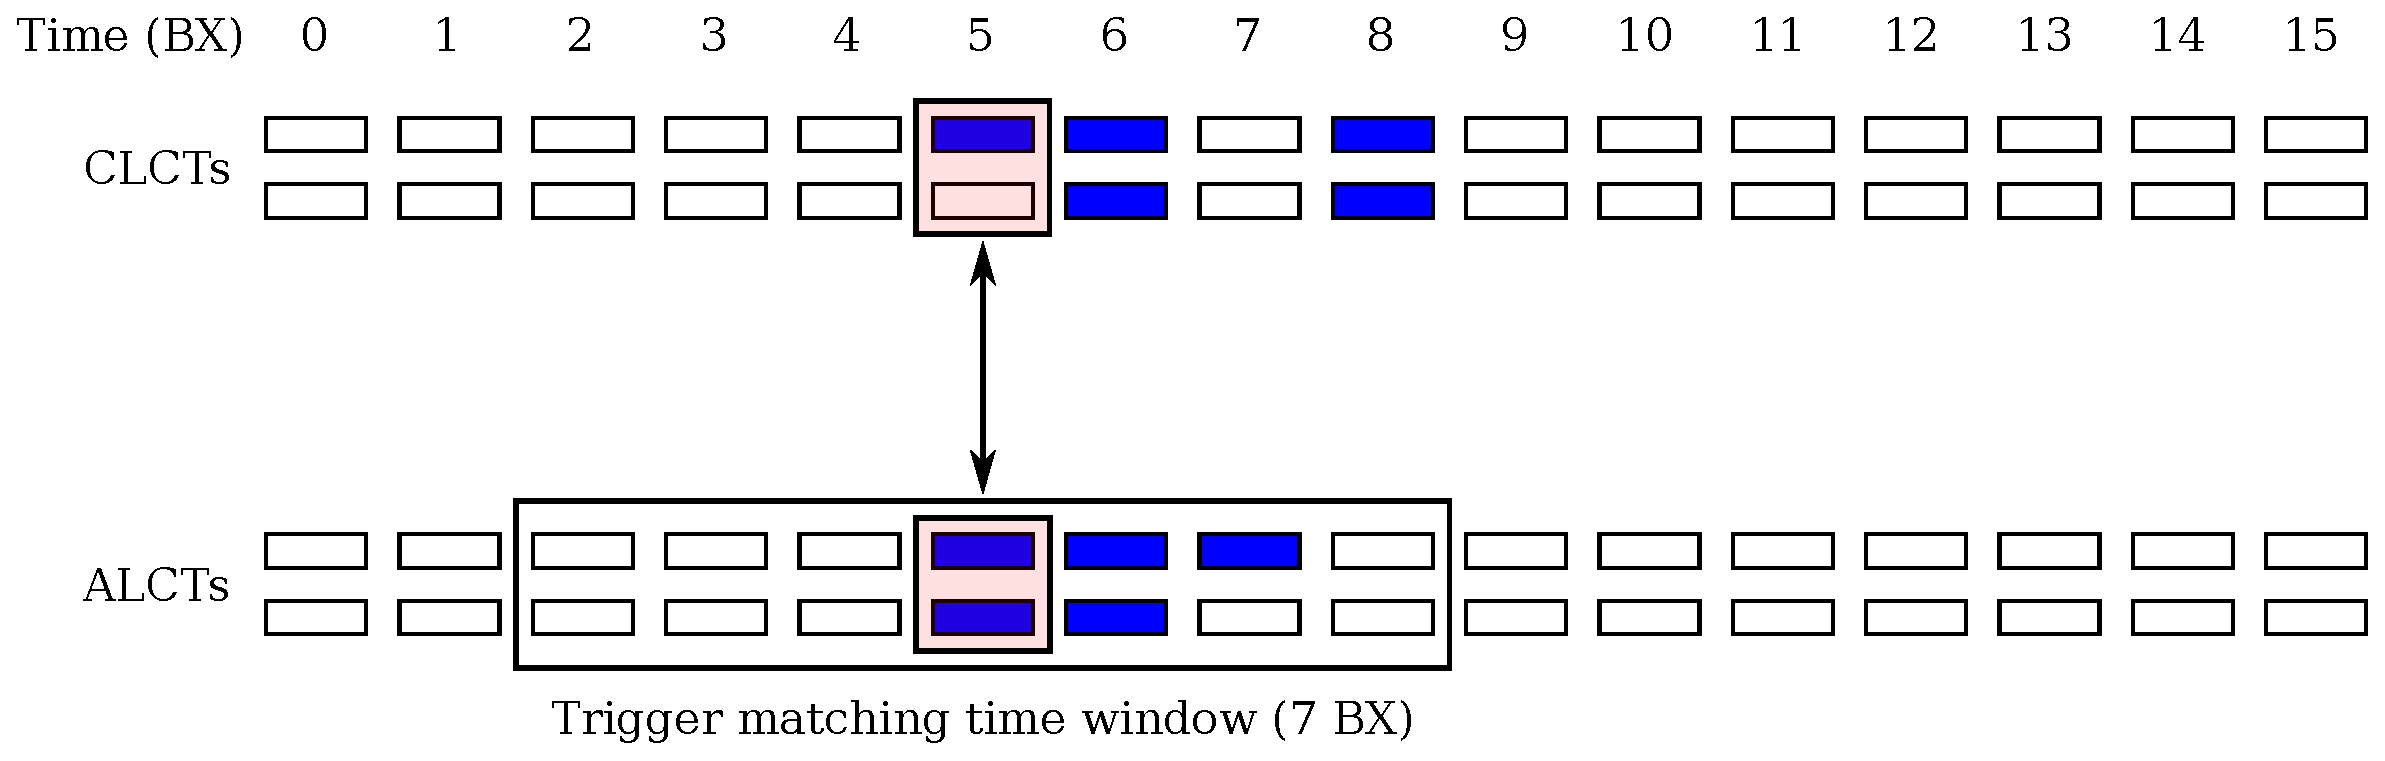
\includegraphics[width=0.7\linewidth]{figures/clct_alcts.pdf}
                \caption{CLCT-centric CLCT and ALCT correlation.}
                \label{fig:clct_alcts}
        \end{center}
\end{figure}

The results of such a correlation are shown on Fig.~\ref{fig:clct_alcts_end}.

\begin{figure}[tbh]
        \begin{center}
                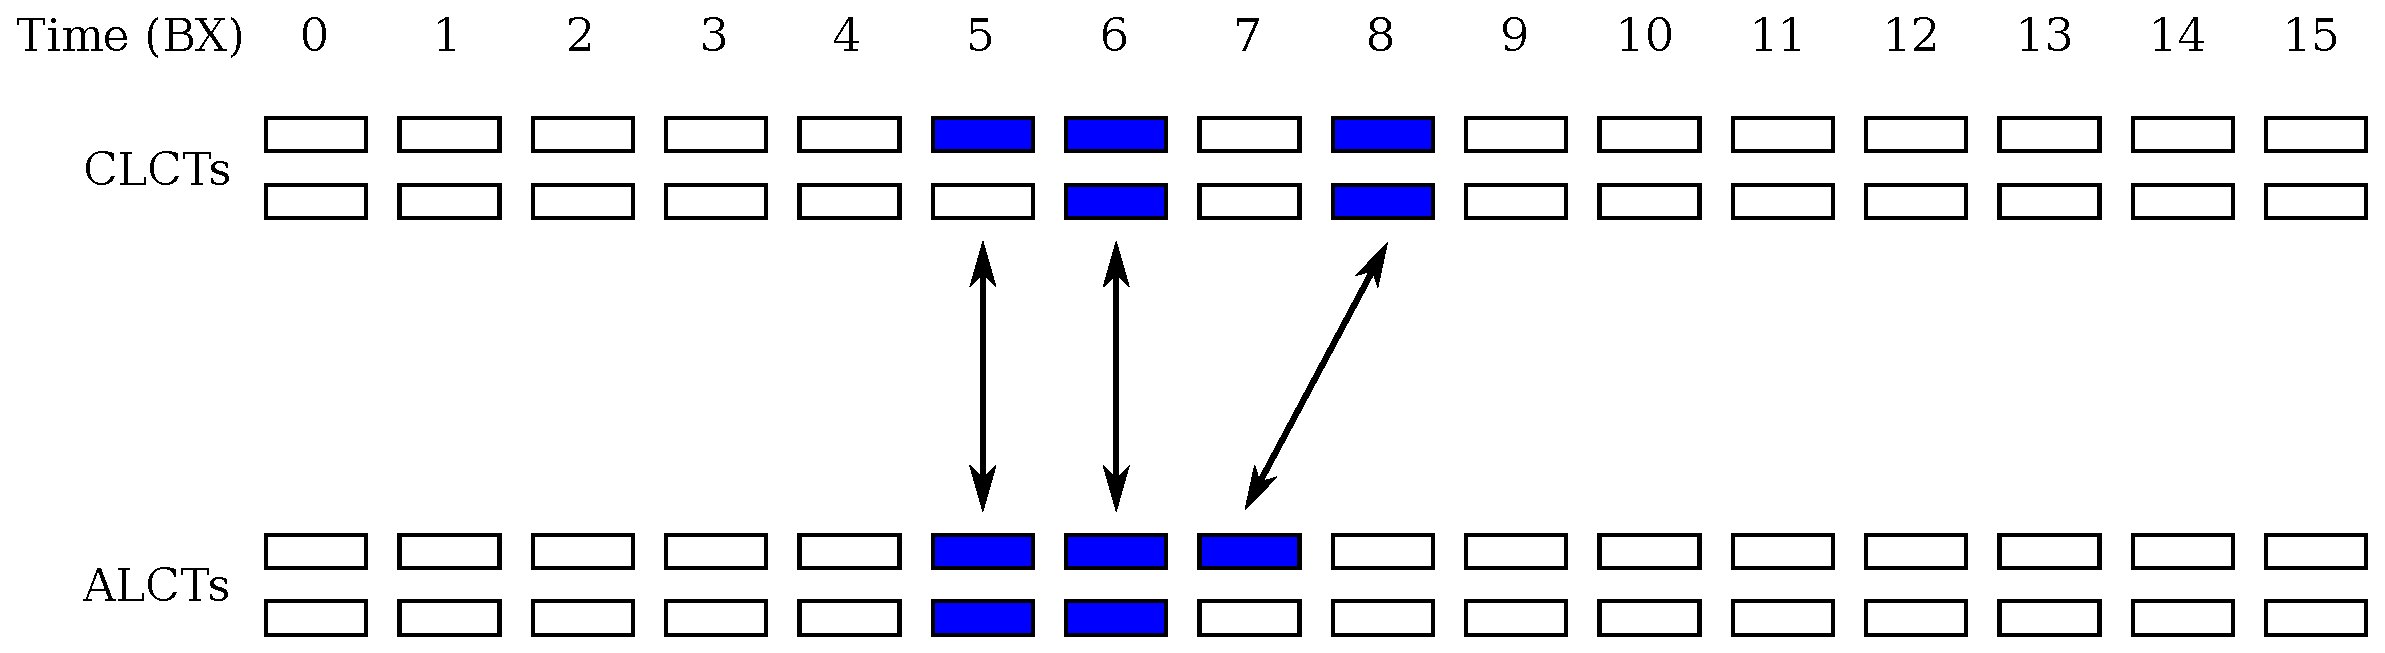
\includegraphics[width=0.7\linewidth]{figures/clct_alcts_end.pdf}
                \caption{Result of CLCT-centric CLCT and ALCT correlation.}
                \label{fig:clct_alcts_end}
        \end{center}
\end{figure}

By default, LCTs are constructed only from valid CLCTs and ALCTs, but we may optionally allow construction of ALCT-less or CLCT-less LCTs.

If there are no ALCT BXs with at least one valid ALCT in the watching window and ALCT-less LCTs are allowed, construct LCTs from valid CLCTs in the current CLCT BX (see example on Fig.~\ref{fig:clct_alcts_alctless} with results on Fig.~\ref{fig:clct_alcts_alctless_end}).

\begin{figure}[tbh]
        \begin{center}
                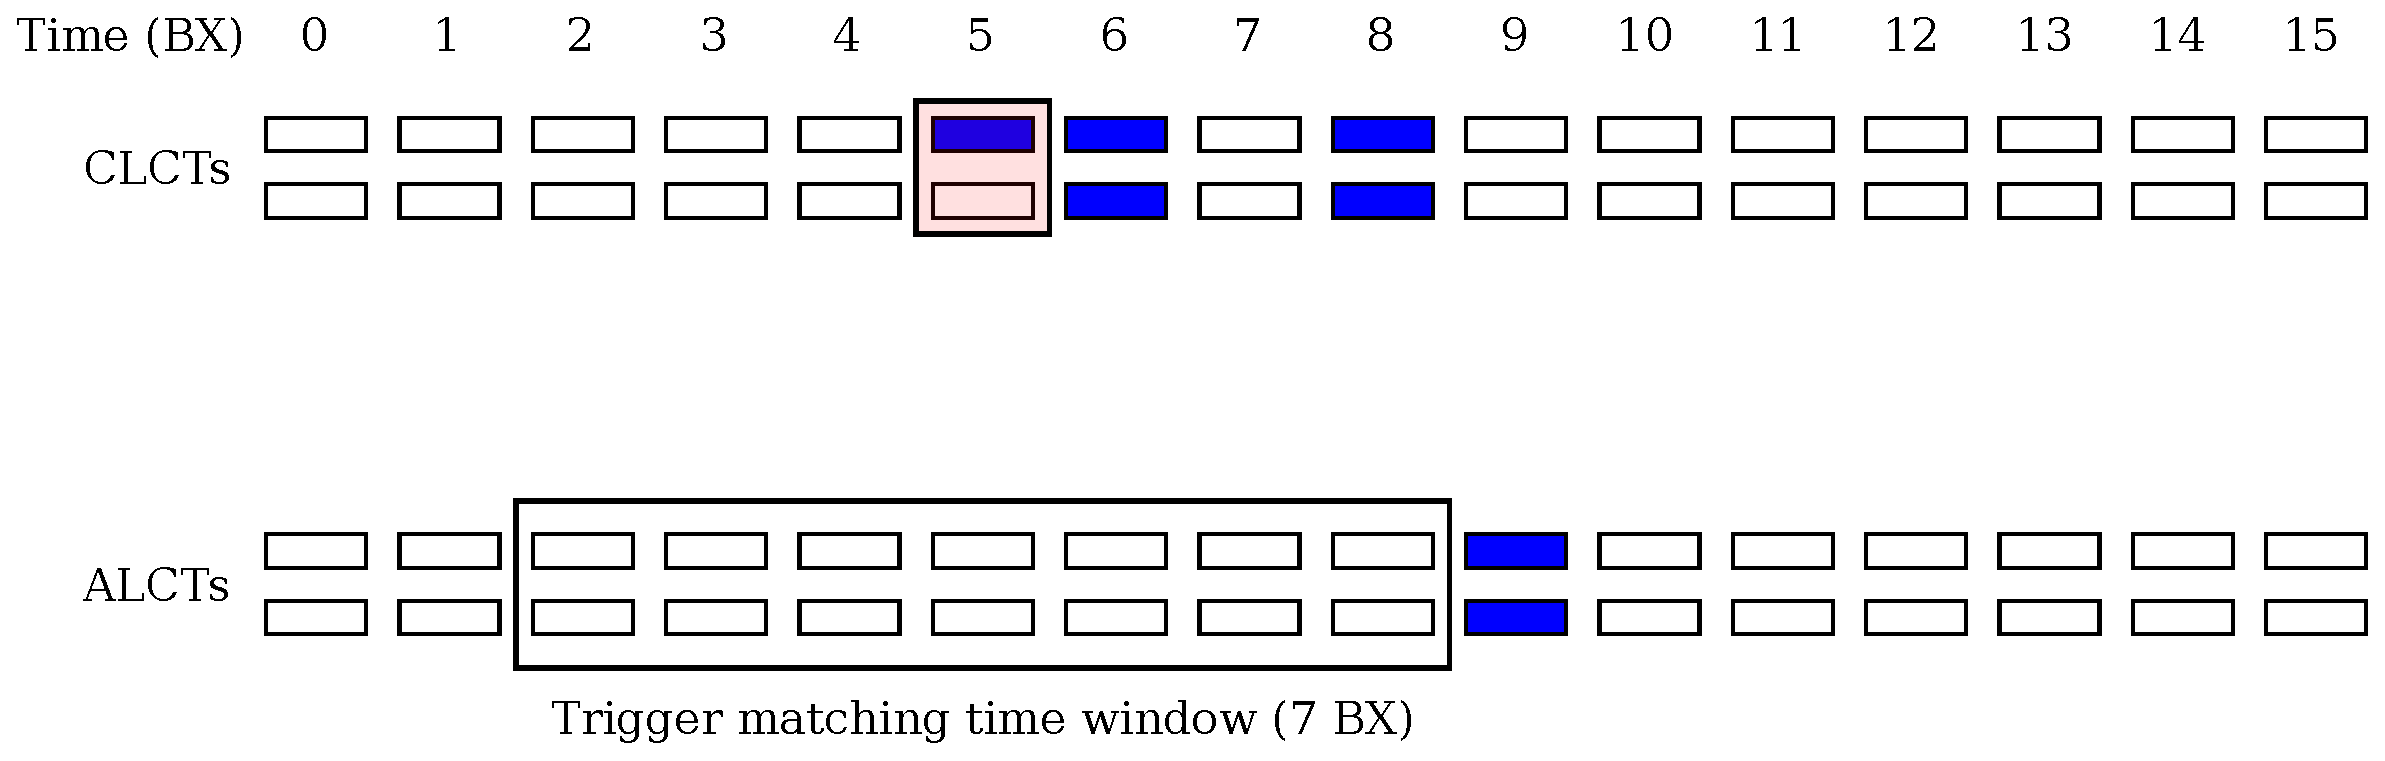
\includegraphics[width=0.7\linewidth]{figures/clct_alcts_alctless.pdf}
                \caption{Example of construction of ALCT-less LCTs.}
                \label{fig:clct_alcts_alctless}
        \end{center}
\end{figure}

\begin{figure}[tbh]
        \begin{center}
                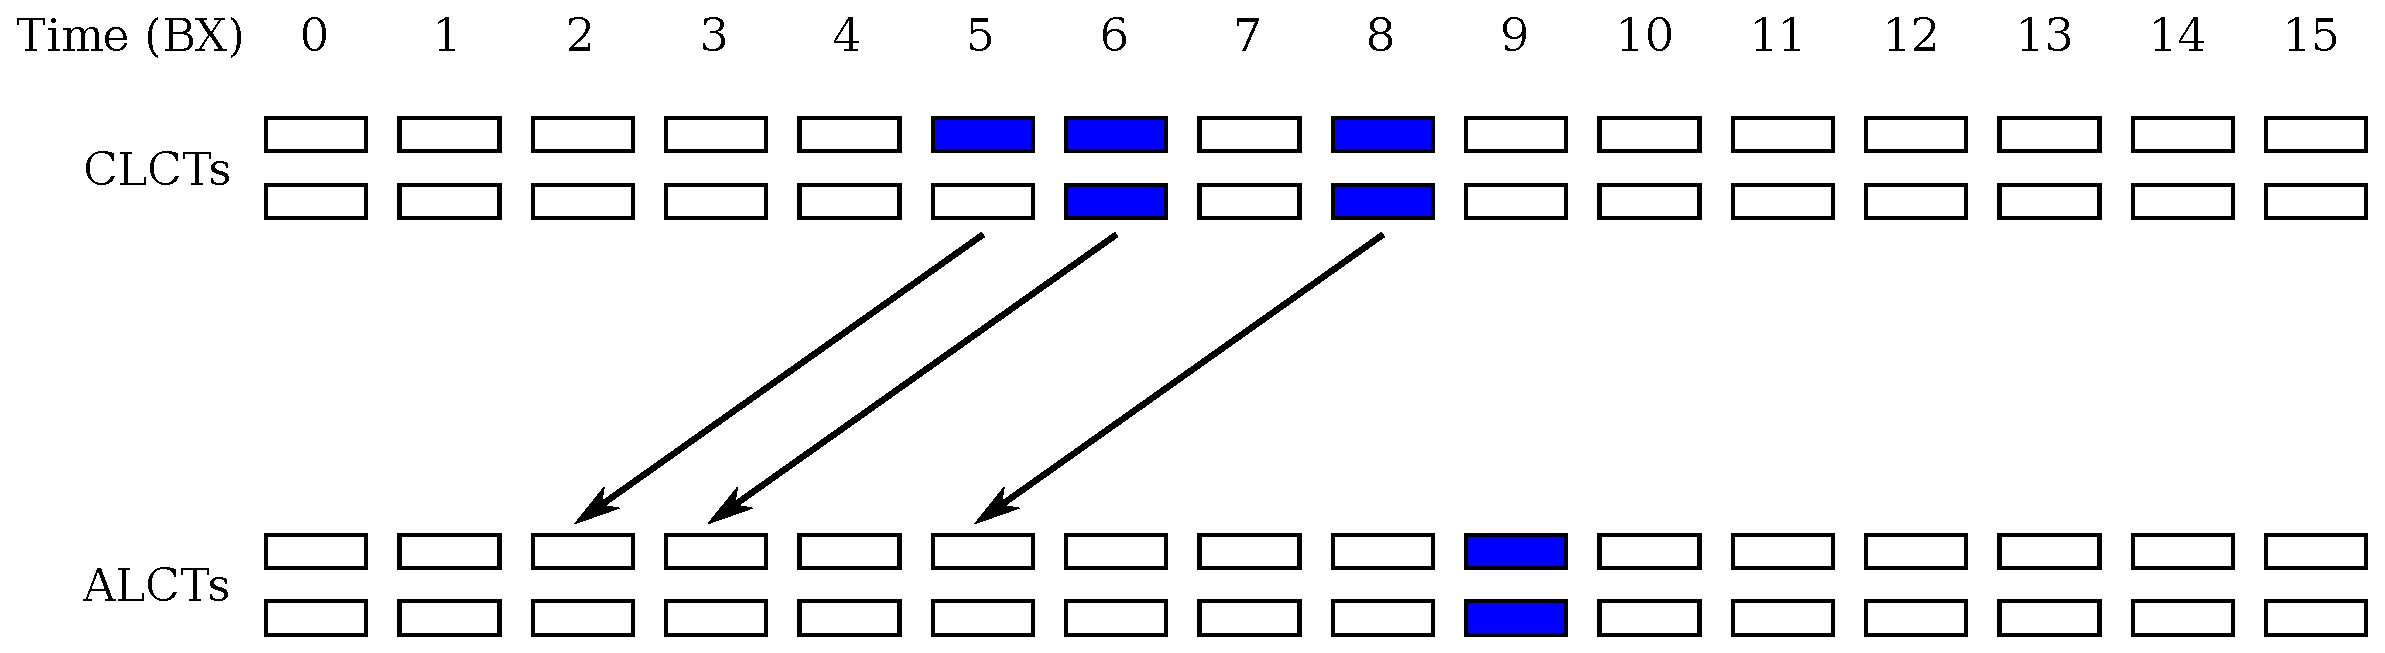
\includegraphics[width=0.7\linewidth]{figures/clct_alcts_alctless_end.pdf}
                \caption{Results of construction of ALCT-less LCTs.}
                \label{fig:clct_alcts_alctless_end}
        \end{center}
\end{figure}

If there are no valid CLCTs in the current CLCT BX and CLCT-less LCTs are allowed (see example on Fig.~\ref{fig:clct_alcts_clctless} with results on Fig.~\ref{fig:clct_alcts_clctless_end}):
\begin{itemize}
    \item Find first ALCT BX in the matching window with at least one valid ALCT and not marked as used before;
    \item Construct LCTs from valid ALCTs in that ALCT BX.
\end{itemize}

\begin{figure}[tbh]
        \begin{center}
                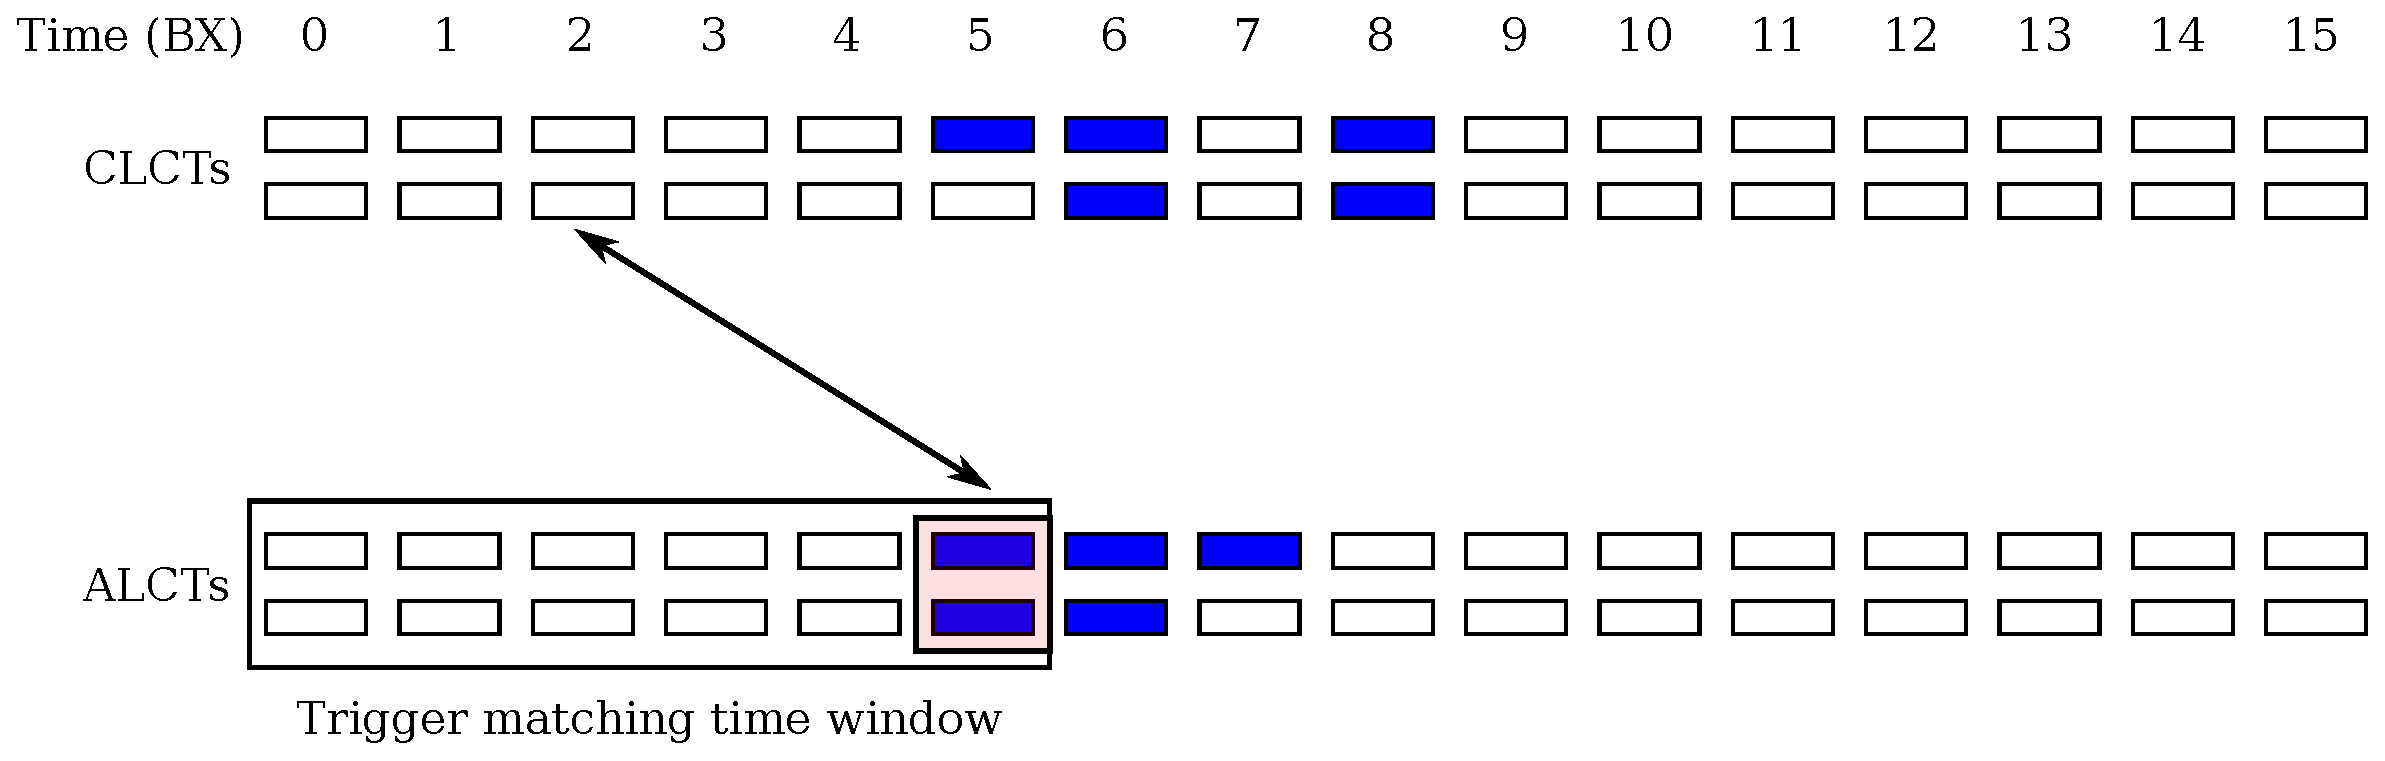
\includegraphics[width=0.7\linewidth]{figures/clct_alcts_clctless.pdf}
                \caption{Example of construction of CLCT-less LCTs.}
                \label{fig:clct_alcts_clctless}
        \end{center}
\end{figure}

\begin{figure}[tbh]
        \begin{center}
                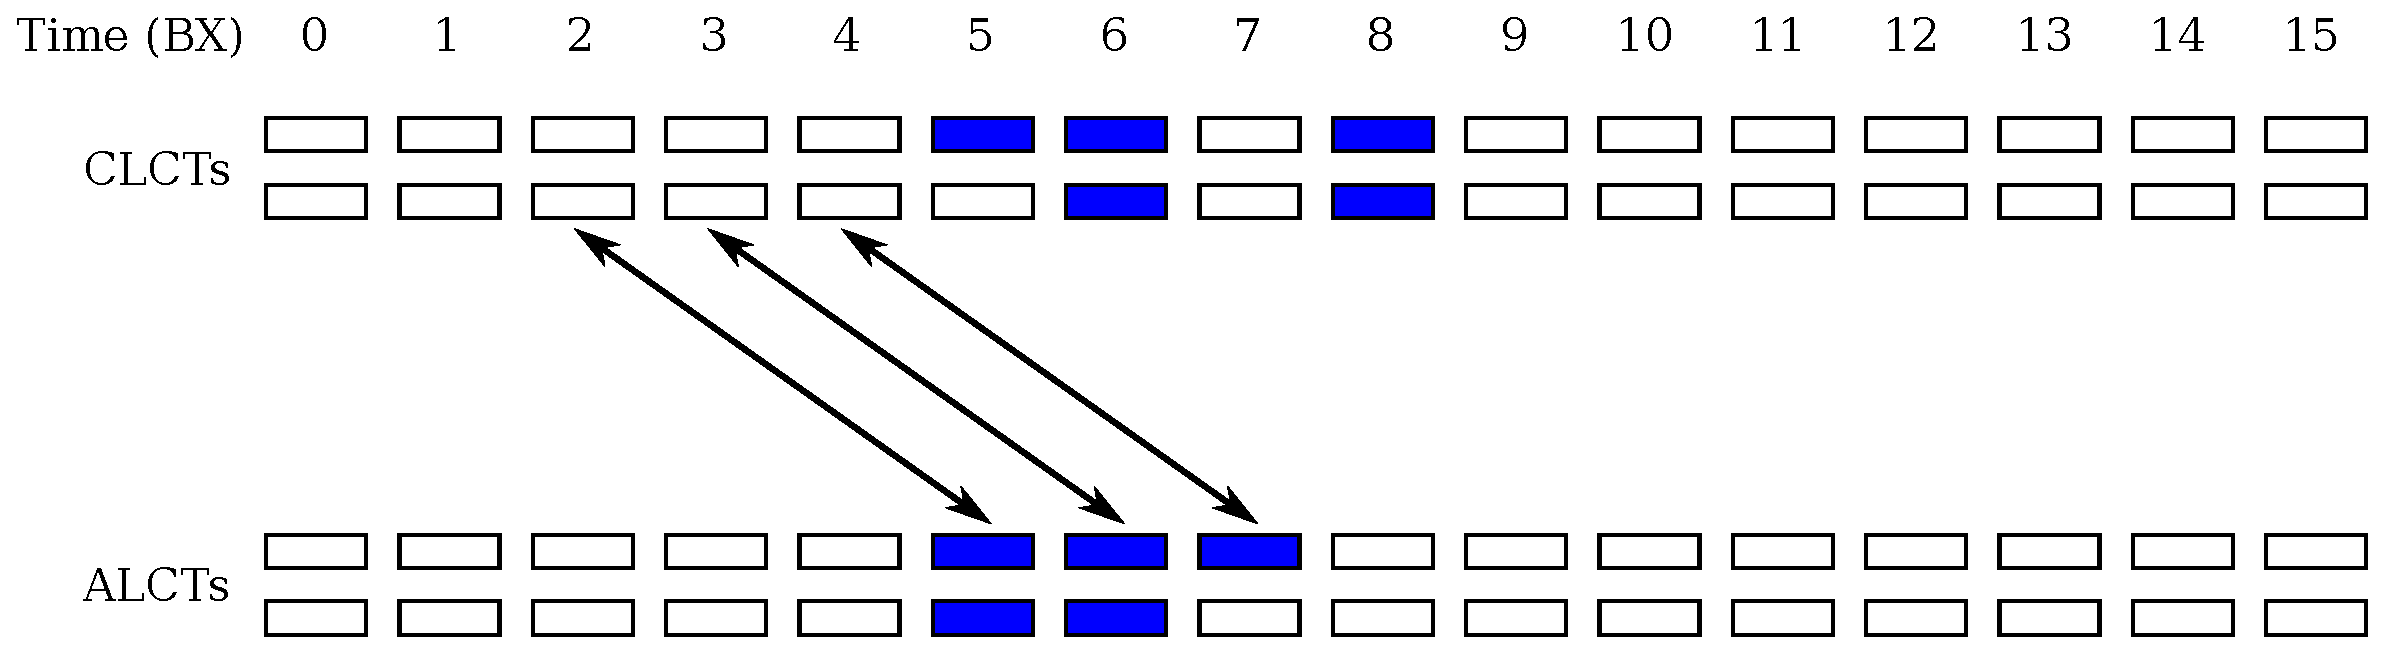
\includegraphics[width=0.7\linewidth]{figures/clct_alcts_clctless_end.pdf}
                \caption{Results of construction of CLCT-less LCTs.}
                \label{fig:clct_alcts_clctless_end}
        \end{center}
\end{figure}

When we use default behavior, where LCTs are constructed only from valid CLCTs and ALCTs, the ideal case is when in matching BXs number of valid CLCTs is equal to number of valid ALCTs (see top two examples on Fig.~\ref{fig:clct_alct_corr}).

\begin{figure}[tbh]
        \begin{center}
                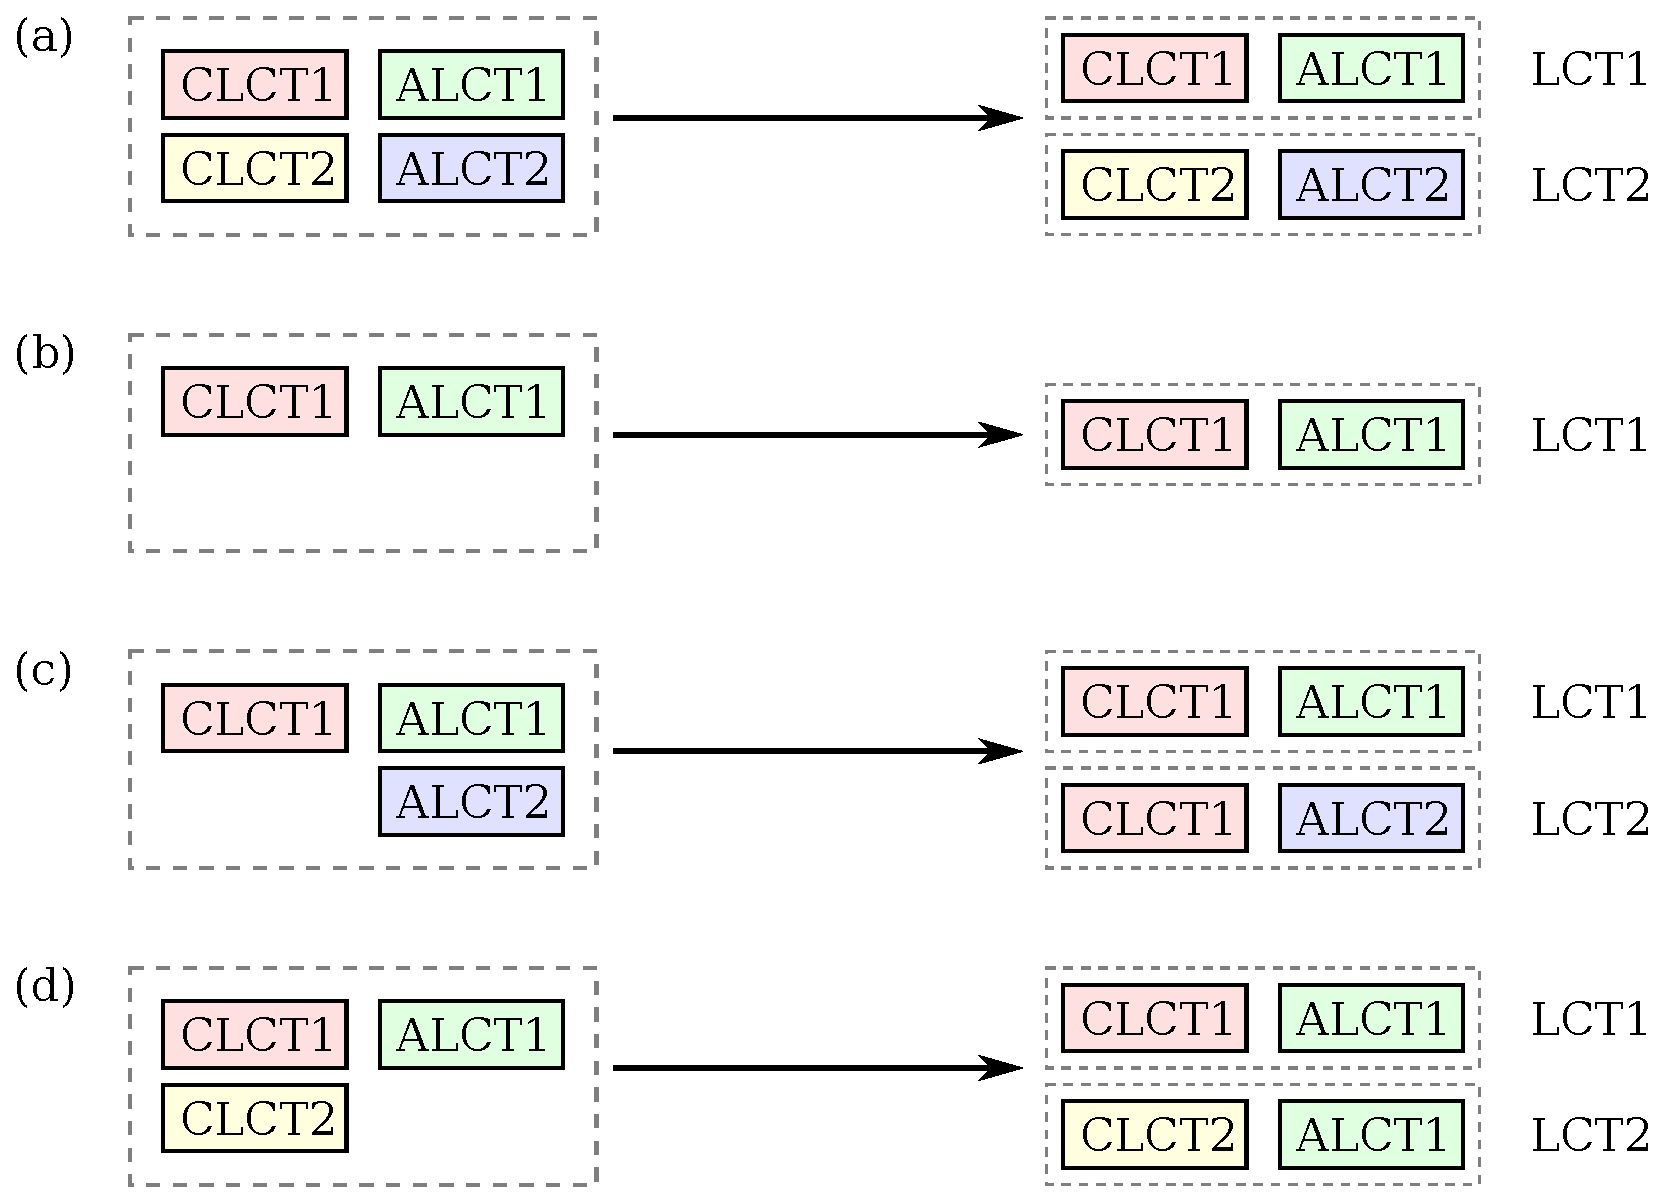
\includegraphics[width=0.7\linewidth]{figures/clct_alct_corr.pdf}
                \caption{Construction of LCTs.}
                \label{fig:clct_alct_corr}
        \end{center}
\end{figure}

But when, for example, there is only one valid CLCT and two valid ALCTs, we make the second valid CLCT from the first, analogously, when there are two valid CLCTs and only one valid ALCT (see bottom two examples on Fig.~\ref{fig:clct_alct_corr}).

\newpage
\subsection{Sofware Emulation of TMB Level Improvements}

\subsubsection{Decreased Trigger Matching Window}

Decrease size of trigger matching time window from 7 BXs to 3 BXs (see Fig.~\ref{fig:clct_alcts_short_window}).

\begin{figure}[tbh]
        \begin{center}
                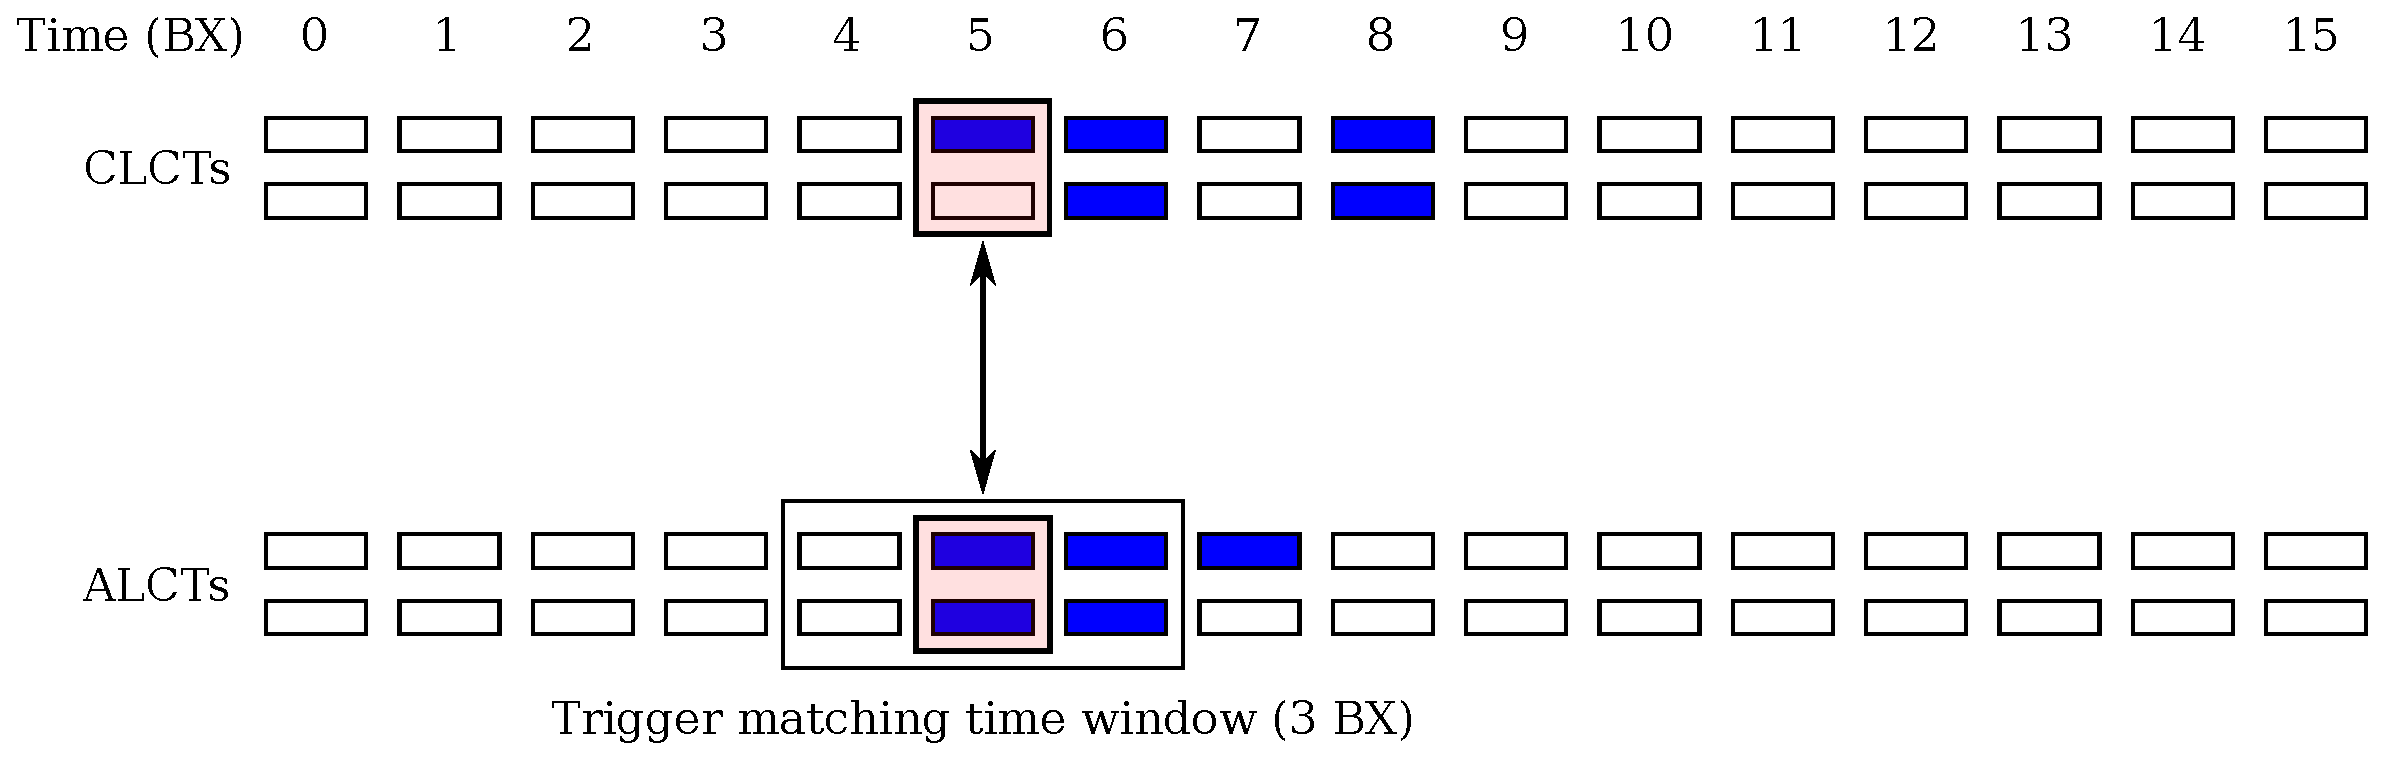
\includegraphics[width=0.98\linewidth]{figures/clct_alcts_short_window.pdf}
                \caption{Decreased trigger matching window.}
                \label{fig:clct_alcts_short_window}
        \end{center}
\end{figure}

The following modifications in configuration are related to this improvement:
\begin{itemize}
    \item matchTrigWindowSize: 7BX to 3BX
\end{itemize}

\subsubsection{ALCT-centric ALCT and CLCT Correlation}

Switch from CLCT-centric matching to ALCT-centric matching (see Fig.~\ref{fig:alct_clcts}).

\textcolor{red}{CLCT-centric matching}
\begin{itemize}
    \item Loop over CLCT BXs from BX = 0 to BX = 15
    \item For CLCT BX = B with at least one valid CLCT:
    \begin{itemize}
        \item Loop over ALCT BXs from BX = B-3 to BX = B+3
    \end{itemize}
\end{itemize}
\textcolor{blue}{ALCT-centric matching}
\begin{itemize}
    \item Loop over ALCT BXs from BX = 0 to BX = 15
    \item For ALCT BX = B with at least one valid ALCT:
    \begin{itemize}
        \item Loop over CLCT BXs from BX = B-3 to BX = B+3
    \end{itemize}
\end{itemize}

\begin{figure}[tbh]
        \begin{center}
                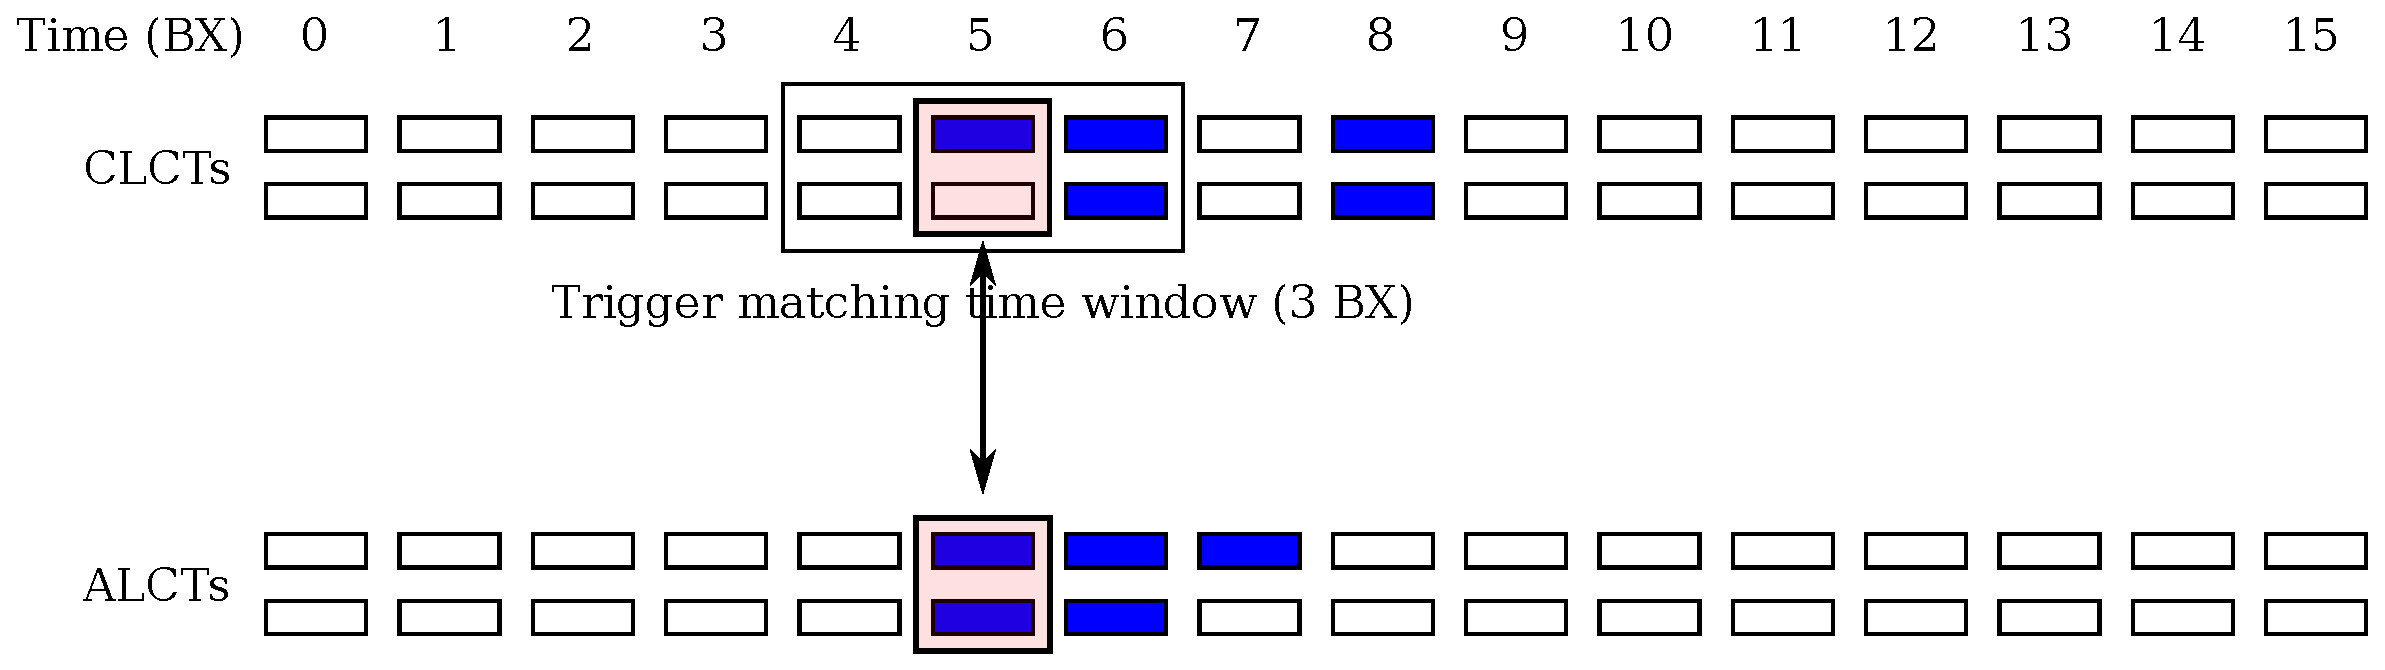
\includegraphics[width=0.98\linewidth]{figures/alct_clcts.pdf}
                \caption{ALCT-centric ALCT anc CLCT correlation.}
                \label{fig:alct_clcts}
        \end{center}
\end{figure}

The following modifications in configuration are related to this improvement:
\begin{itemize}
    \item clctToAlct: True to False
\end{itemize}

\subsubsection{Reusage of Used ALCTs and CLCTs}

Allow reusage of ALCTs and CLCTs already used during ALCT and CLCT correlation (see Fig.~\ref{fig:reuse_alct_clct}).

\textcolor{red}{Current behavior}:
\begin{itemize}
    \item Drop used CLCTs: do not use them with ALCTs in other ALCT BXs;
    \item Proceed to next ALCT BX after matching ALCTs with earliest CLCT BX with at least one valid CLCT.
\end{itemize}
\textcolor{blue}{New behavior}:
\begin{itemize}
    \item Do not drop used CLCTs: reuse them with ALCTs in other ALCT BXs;
    \item Match ALCTs to CLCTs in all CLCT BXs within matching window.
\end{itemize}

\begin{figure}[tbh]
        \begin{center}
                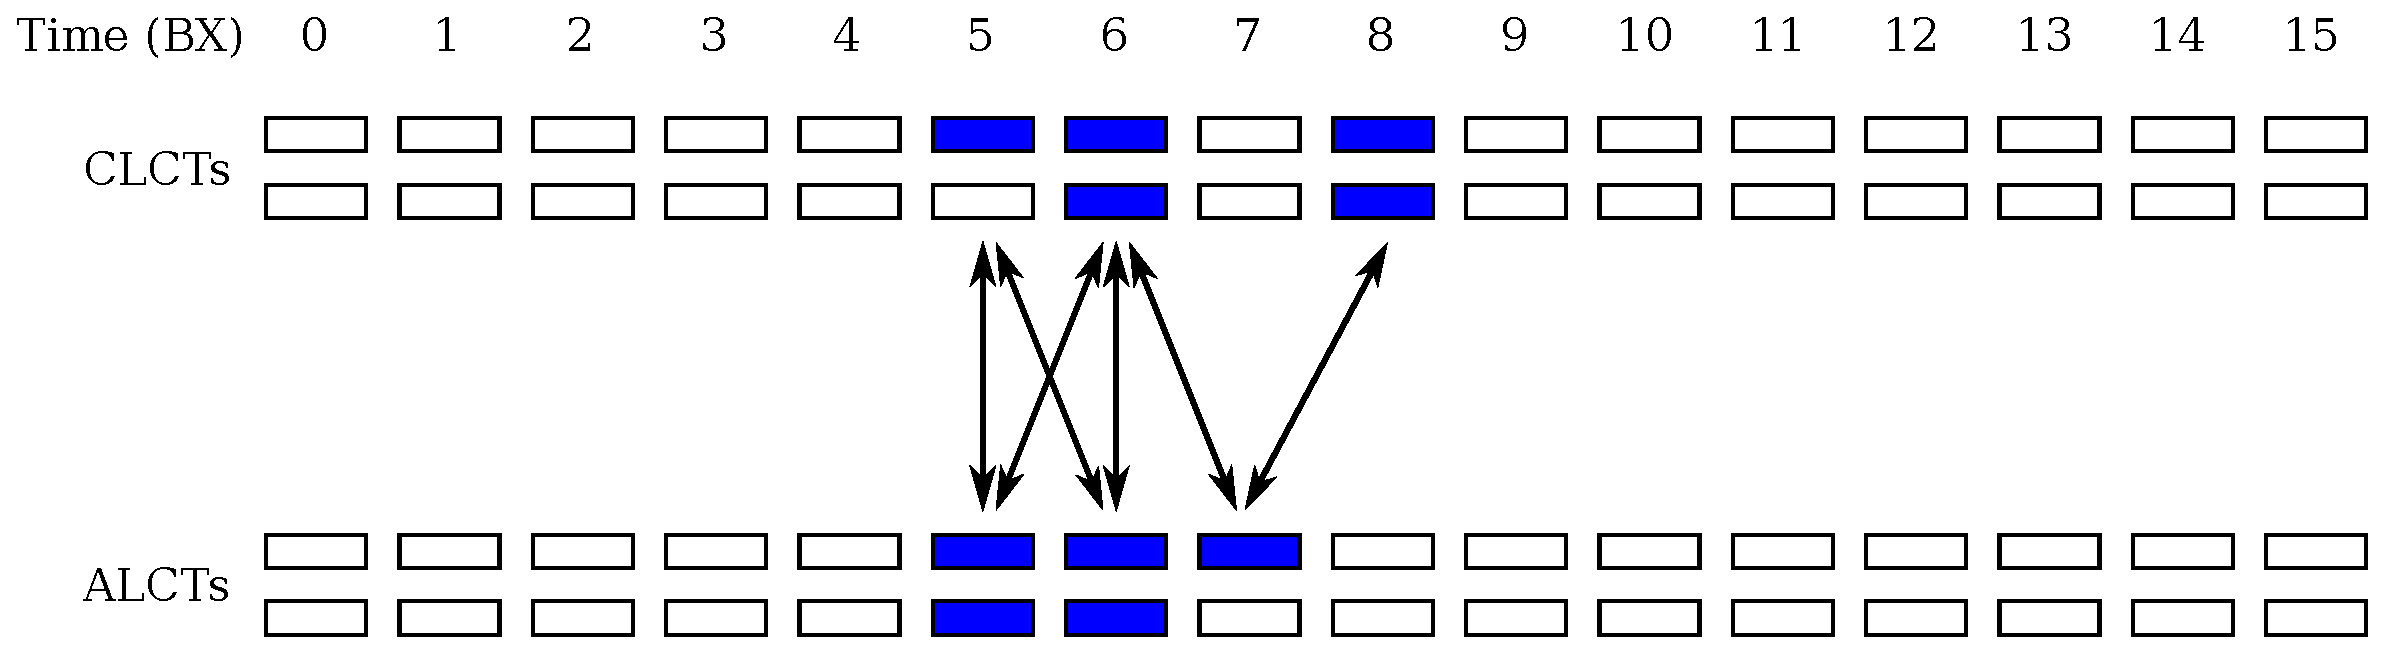
\includegraphics[width=0.98\linewidth]{figures/clct_alcts_end_2.pdf}
                \caption{Reusage of already used ALCTs and CLCTs.}
                \label{fig:reuse_alct_clct}
        \end{center}
\end{figure}

The following modifications in configuration are related to this improvement:
\begin{itemize}
    \item tmbDropUsedClcts: True to False
    \item matchEarliestClctME11Only: True to False
\end{itemize}

\subsubsection{Cross BX Algorithm}

In the situation shown on Fig.~\ref{fig:reuse_alct_clct}, in some given BX = B we can end up having with up to 6 LCTs (made from ALCTs in BX = B and CLCTs in BX = B-1, B, B+2. How do we choose two LCTs to be reported for BX = B?

\textcolor{red}{Current behavior: "cross bx" algorithm is turned off}
\begin{itemize}
    \item Choose two best LCTs with the highest quality
\end{itemize}
\textcolor{blue}{New behavior: "cross bx algorithm"}
\begin{itemize}
    \item Take LCTs with ALCT BX = B and CLCT BX = B
    \item If we still don't have two LCTs, take best ones with ALCT BX = B-1
    \item If we still don't have two LCTs, take best ones with ALCT BX = B+1
\end{itemize}

The following modifications in configuration are related to this improvement:
\begin{itemize}
    \item tmbCrossBxAlgorithm: 0 to 1
\end{itemize}

\newpage

\subsubsection{Corrected ALCT and CLCT Timing}

Use more robust procedure for assignment of ALCT BX and CLCT BX.

\textcolor{red}{Current behavior}:
\begin{itemize}
    \item Use ALCT and CLCT pretrigger BXs to assign ALCT BX and CLCT BX.
\end{itemize}
\textcolor{blue}{New behavior}:
\begin{itemize}
    \item For each hit in ALCT and CLCT trigger patterns, determine "first BX": BX of original hit before hit stretching over 6 BXs;
    \item For ALCTs, consider hits in key WG = N and two neighbouring WGs: WG = N-1 and WG = N+1;
    \item For CLCTs, consider all hits in the pattern;
    \item Store "first BXs" of these hits in two sorted sets (one for ALCT times and another for CLCT times);
    \item Use median elements in these sets to assign ALCT BX and CLCT BX.
\end{itemize}

The following modifications in configuration are related to this improvement:
\begin{itemize}
    \item alctUseCorrectedBx: False to True
    \item clctUseCorrectedBx: False to True
\end{itemize}

\subsubsection{Reading out more LCTs}

[I'm not sure I completely understand the meaning of this improvement]

\textcolor{red}{Current behavior}
\begin{itemize}
    \item In digi$\rightarrow$raw step, LCTs have to be packed into the TMB header, and currently there is room just for two
    \item Take LCTs only from earliest BX in L1A readout with at least one LCT
\end{itemize}
\textcolor{blue}{New behavior}
\begin{itemize}
    \item Take LCTs from the whole L1A readout (from BX = 5 to BX = 11)
\end{itemize}

The following modifications in configuration are related to this improvement:
\begin{itemize}
    \item tmbReadoutEarliest2: True to False
\end{itemize}


\subsection{Results of Improvements of the ALCT and CLCT Matching}

Improvements on the level of TMB are related to the following configuration parameters (see Sec.~\ref{sec:TMB_conf}):
\begin{itemize}
	\item matchTrigWindowSize: 7BX to 3BX;
	\item tmbReadoutEarliest2: True to False;
	\item alctUseCorrectedBx: False to True
	\item clctUseCorrectedBx: False to True;
	\item clctToAlct: True to False;
	\item tmbDropUsedClcts and matchEarliestClctME11Only: True to False;
	\item tmbCrossBxAlgorithm: 0 to 1.
\end{itemize}

Fig.~\ref{fig:TMB_improvements_LCT_recoEff} shows reconstruction efficiency of a good LCT in ME1/1 station versus pseudorapidity of the simulated muon for different L1 configurations. The good LCT is defined as LCT consisted of a good ALCT and a good CLCT.

The major improvement in LCT reconstruction efficiency comes from:
\begin{itemize}
	\item changing the size of a window where ALCTs and CLCTs are read out for further correlation between each other;
	\item stopping to read out only the first two CLCTs;
	\item stopping to drop used CLCTs;
	\item stopping to match only to the earliest CLCT.
\end{itemize}

The effects on the efficiency improvements are more evident if we divide the whole ME1/1 chamber into three different sections by eta:
\begin{itemize}
        \item from $ \eta = 1.65 $ to $ \eta = 2.0 $ to cover the ME1/1b chamber alone;
        \item from $ \eta = 2.0 $ to $ \eta = 2.2 $ to cover the gap between ME1/1a and ME1/1b;
        \item from $ \eta = 2.2 $ to $\eta = 2.45 $ to cover the ME1/1a chamber alone;
\end{itemize}

The effects on the efficiency for each one of the TMB improvment in the main $\eta$ partitions defined above are summarized in Tab.~\ref{eff_pu140} for PU140 and in Tab.~\ref{eff_pu50} for PU50. A more detailed study comparing each improvment over the whole $\eta$ range for the ME1/1 chamber can be found in Appendix.

\begin{figure}[p]
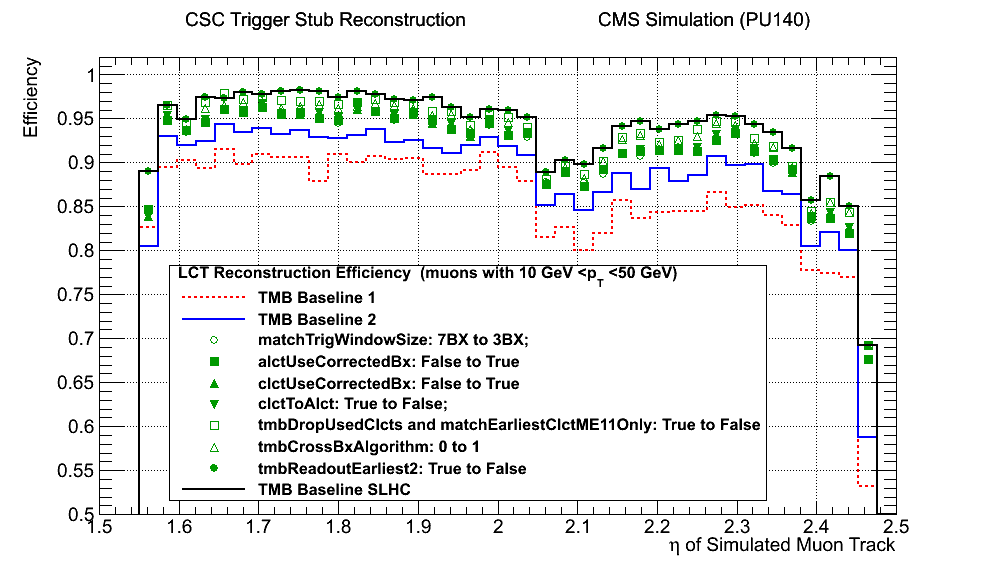
\includegraphics[width=0.98\textwidth]{figures/TMB_improvements_LCT_recoEff.png}
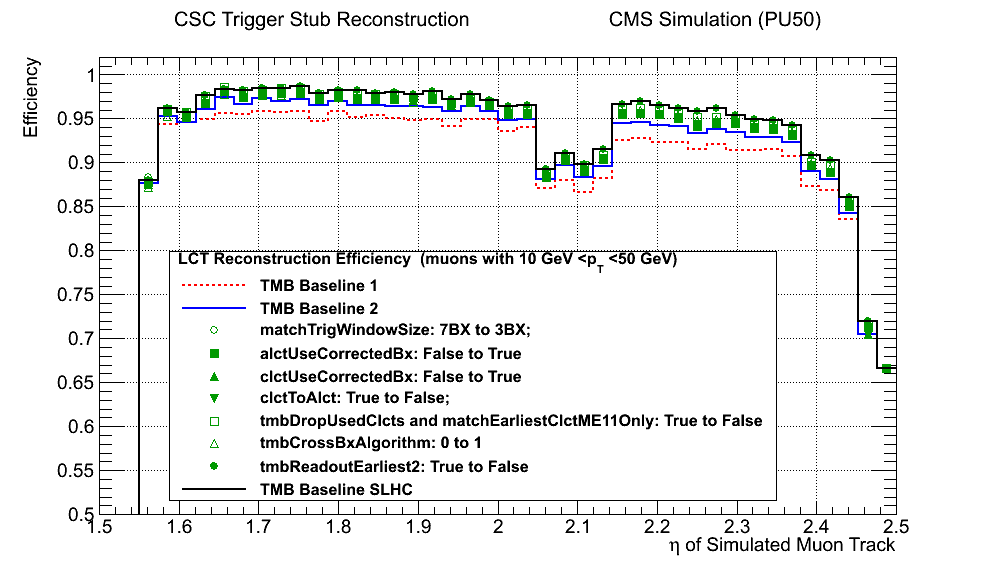
\includegraphics[width=0.98\textwidth]{figures/TMB_improvements_LCT_recoEff_PU50.png}
\caption{LCT reconstruction efficiency in ME1/1 station for PU140 (top) and PU50 (bottom). Muons with transverse momentum $10$~GeV$<p_T<50$~ GeV are used in the analysis.}
\label{fig:TMB_improvements_LCT_recoEff}
\end{figure}

\begin{table}[h]
\begin{tabular}{| p{7.4 cm}| c | c | c | c | c | c | }
\hline
\multirow{2}{*}{Improvment} & \multicolumn {2}{|c|}{ME1/1b} & \multicolumn{2}{|c|}{Gap Region} & \multicolumn{2}{|c|}{ME1/1a} \\ \cline{2-7}
                            & $\epsilon$ (\%)  & $\delta \epsilon$ & $\epsilon$ (\%) & $\delta \epsilon$ & $\epsilon$ (\%) & $\delta \epsilon$ \\  \hline
TMB Baseline 1 & 89.92 & 0.13 & 82.62 & 0.16 & 82.54 & 0.16 \\ \hline
TMB Baseline 2 & 92.63 & 0.11 & 86.53 & 0.15 & 86.38 & 0.15 \\ \hline
matchTrigWindowsSize: 7BX to 3 BX & 94.38 & 0.09 & 89.27 & 0.13 & 88.97 & 0.13 \\ \hline
alctUseCorrectedBX: False to True & 95.00 & 0.09 & 89.36 & 0.13 & 89.35 &  0.13  \\ \hline 
clctUseCorrectedBX: False to True & 95.01 & 0.09 & 89.37 & 0.13 & 89.36 & 0.13 \\ \hline
clctToAlct: True to False & 95.11 & 0.09 & 89.40 & 0.13 & 80.36 & 0.13 \\ \hline
tmbDropUsedClcts and matchEarliestClctME11Only: False to True & 96.27 & 0.08 & 90.54 & 0.12 & 90.59 & 0.12 \\ \hline
tmbCrossBXAlgorithm: 0 to 1 & 95.69 & 0.09 & 90.24 & 0.13 & 90.33 & 0.13 \\ \hline
tmbReadoutEarliest2: True to False & 97.00 & 0.07 & 91.65 & 0.12 & 91.97 & 0.12 \\ \hline
TMB Baseline SLHC & 97.00 & 0.07 & 91.65 & 0.12 & 91.97 & 0.12 \\ \hline
\end{tabular}
\caption{LCT reconstruction efficiencies in ME1/1 station after individual improvements in algorithm for PU140. Muons with transverse momentum $10$~GeV$<p_T<50$~ GeV are used in the analysis.}
\label{eff_pu140}
\end{table}

\begin{table}[h]
\begin{tabular}{| p{7.4 cm}| c | c | c | c | c | c | }
\hline
\multirow{2}{*}{Improvment} & \multicolumn {2}{|c|}{ME1/1b} & \multicolumn{2}{|c|}{Gap Region} & \multicolumn{2}{|c|}{ME1/1a} \\ \cline{2-7}
                            & $\epsilon$ (\%)  & $\delta \epsilon$ & $\epsilon$ (\%) & $\delta \epsilon$ & $\epsilon$ (\%) & $\delta \epsilon$ \\  \hline
TMB Baseline 1 & 94.95 & 0.09 & 89.18 & 0.13 & 90.38 & 0.13 \\ \hline
TMB Baseline 2 & 96.32 & 0.08 & 90.74 & 0.12 & 91.78 & 0.12 \\ \hline
matchTrigWindowsSize: 7BX to 3 BX & 97.13 & 0.07 & 91.72 & 0.12 & 92.91 & 0.11 \\ \hline
alctUseCorrectedBX: False to True & 97.13 & 0.07 & 91.80 & 0.12 & 93.00 & 0.11 \\ \hline
clctUseCorrectedBX: False to True & 97.03 & 0.07 & 91.80 & 0.12 & 93.06 & 0.11 \\ \hline
clctToAlct: True to False & 97.03 & 0.07 & 91.80 & 0.12 & 93.06 & 0.11 \\ \hline
tmbDropUsedClcts and matchEarliestClctME11Only: False to True & 97.52 & 0.07 & 92.23 & 0.11 & 93.61 & 0.10 \\ \hline
tmbCrossBXAlgorithm: 0 to 1 & 97.03 & 0.07 & 91.86 & 0.12 & 93.39 & 0.11 \\ \hline
tmbReadoutEarliest2: True to False & 97.69 & 0.06 & 92.62 & 0.11 & 94.07 & 0.10 \\ \hline 
TMB Baseline SLHC & 97.69 & 0.06 & 92.62 & 0.11 & 94.07 & 0.10 \\ \hline 
\end{tabular}
\caption{LCT reconstruction efficiencies in ME1/1 station after individual improvements in algorithm for PU50. Muons with transverse momentum $10$~GeV$<p_T<50$~ GeV are used in the analysis.}
\label{eff_pu50}
\end{table}
